\subsection{Merkle Tree on Blockchain}
Merkle trees on the blockchain are binary trees that are used to store transaction information. Figure 2 shows the structure of a Merkle hash tree on the blockchain. Each transaction in the figure is paired two by two to form the leaf nodes of the Merkle tree, which in turn generates the entire Merkle tree. 
\begin{figure}[H]
    \centering
    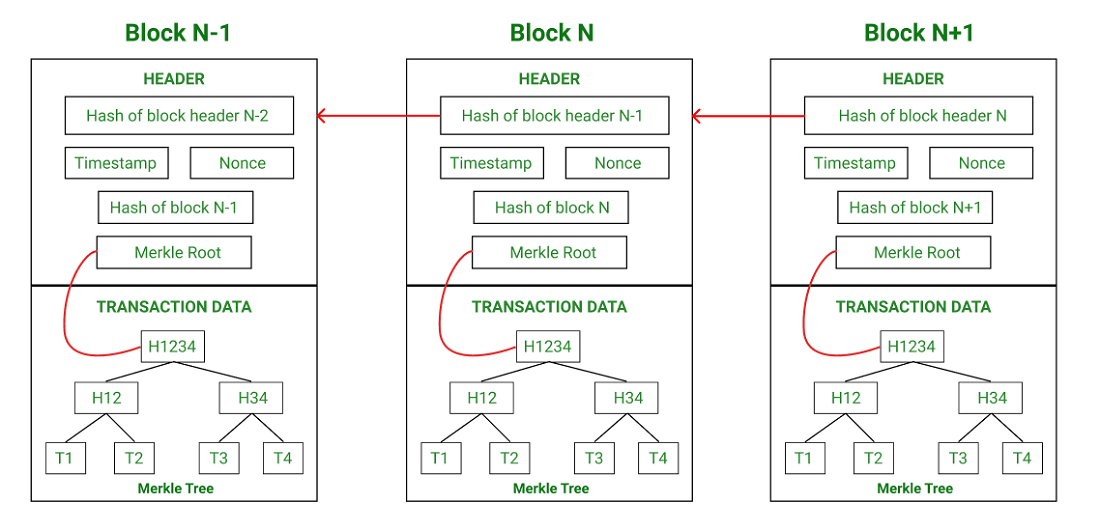
\includegraphics[scale=0.6]{figures/Blockchain and Merkle Tree.png}
    \caption{Merkle Tree on Blockchain}
 
\end{figure}
The Merkle tree allows a client to verify whether the transaction is included in a block by using the Merkle tree root obtained from the block header and a list of intermediate hashes provided by other clients. The client providing the intermediate hashes does not need to be trustworthy since forging the block header is expensive, and forging the intermediate hashes would cause the verification to fail.
In Merkle tree and blockchain scheme, the Merkle tree is used to store and verify the integrity of data, while the blockchain is used to store and verify the authenticity of the data.
As we know, Merkle Hash Tree is one of the critical technologies of blockchain. It does not require downloading all transaction data to verify data integrity. Although the Merkle tree structure has outstanding advantages, its linear structure and a large number of hash operations make the processing speed not very satisfactory, and the value of each node in the binary tree structure also needs to be stored, which generates a large amount of storage overhead.
